\section{Observed California fixed-backbone inhibition}

\label{sec:s04-observed-completed}

The observed comparison uses the same three California folds and 315 targets. Background and excitation nuisance inputs are fixed and shared between each candidate and its exact uninhibited floor. The common mark term cancels from each held-out joint gain, reported as floor NLL minus selected NLL.

Original LI is retained unpenalized. Magnitude-scaled LI+ is evaluated with immigrant-only and total-intensity attenuation, each with raw training selection and with the declared training-only BIC-style gate. A gate may select the exact floor. A negative held-out gain is retained, while an unresolved numerical result remains unknown rather than being assigned zero.

Table~\ref{tab:s04-observed} reports the three active empirical contrasts. Table~\ref{tab:s04-observed-boundary} partitions the twelve gate-selected or nested rows whose training solution is $\hat\eta=0$: for these cells the held-out joint contrast is identically $0.0000$ by algebraic nesting, not an independent empirical test of zero attenuation. Presenting the twelve zero rows as separate powered comparisons would overstate the evidence.

\begin{table}[htbp]\centering\caption{Active held-out joint gains (nats) relative to the shared uninhibited floor. All three rows select positive total-intensity attenuation in training and lose held-out joint score. Displayed values are empirical contrasts, not algebraic returns. Paired block intervals for raw total-intensity attenuation are reported in Section~\ref{sec:li-score-uncertainty}.}\label{tab:s04-observed}

\begin{tabular}{llllrll}\toprule Fold & Model & Gate & Status & Gain & Win & Active\\\midrule

0 & LI+ total & raw & resolved & -0.2245 & no & yes \\

1 & LI+ total & raw & resolved & -1.9529 & no & yes \\

2 & LI+ total & raw & resolved & -0.2093 & no & yes \\

\bottomrule\end{tabular}\end{table}

\begin{table}[htbp]\centering\caption{Boundary-selected rows partitioned from the active contrasts. Each displayed $0.0000$ is the exact algebraic forecast of the nested $\hat\eta=0$ floor, not an estimate of a zero physical effect. The twelve cells are three folds of four floor-selected procedures and must not be counted as twelve independent empirical test contrasts.}\label{tab:s04-observed-boundary}

\begin{tabular}{llllr}\toprule Fold & Model & Gate & Status & Algebraic gain\\\midrule

0 & LI & raw & floor-selected & 0.0000 \\

0 & LI+ immigrant & raw & floor-selected & 0.0000 \\

0 & LI+ immigrant & BIC & floor-selected & 0.0000 \\

0 & LI+ total & BIC & floor-selected & 0.0000 \\

1 & LI & raw & floor-selected & 0.0000 \\

1 & LI+ immigrant & raw & floor-selected & 0.0000 \\

1 & LI+ immigrant & BIC & floor-selected & 0.0000 \\

1 & LI+ total & BIC & floor-selected & 0.0000 \\

2 & LI & raw & floor-selected & 0.0000 \\

2 & LI+ immigrant & raw & floor-selected & 0.0000 \\

2 & LI+ immigrant & BIC & floor-selected & 0.0000 \\

2 & LI+ total & BIC & floor-selected & 0.0000 \\

\bottomrule\end{tabular}\end{table}

The BIC-style gate is a complexity penalty, not a Davies-calibrated test or a guarantee of nominal size. A training-active fit, a selected floor and a held-out win are distinct outcomes. These observed folds have been inspected retrospectively.

\begin{figure}[p]\centering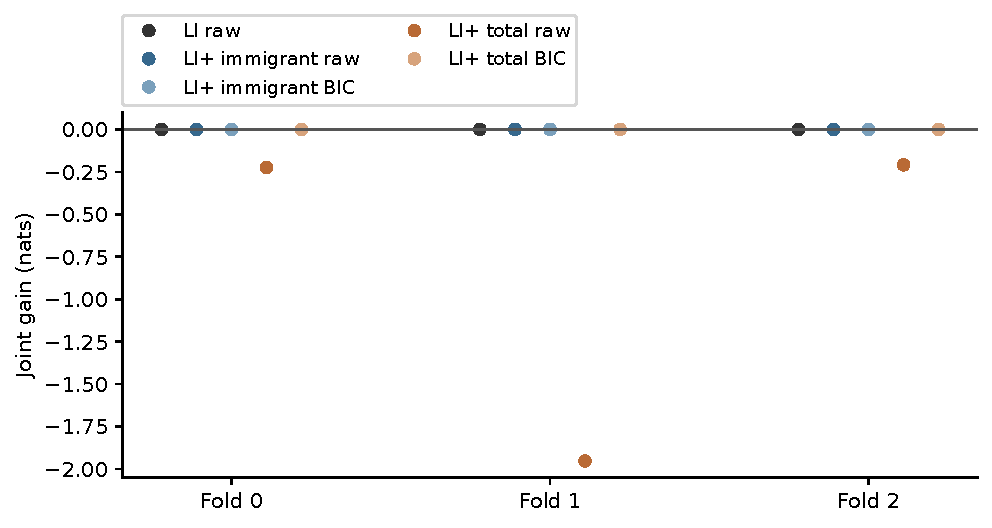
\includegraphics[width=\textwidth]{s04_observed_joint_gains.pdf}\caption{Held-out joint gains on the fixed three-fold population.}\end{figure}

\begin{center}\begin{tabular}{lrr}\toprule Fold & Training targets & Planned held-out targets\\\midrule

0 & 851 & 79 \\

1 & 930 & 167 \\

2 & 1097 & 69 \\

\bottomrule\end{tabular}\end{center}

All original LI and magnitude-scaled immigrant-only fits select their exact uninhibited floor. Raw total-intensity inhibition is active but loses held-out joint score in each fold. Its BIC-gated version selects the floor in every fold. These outcomes do not establish a predictive benefit from the revised inhibition mechanisms on this fixed observed population.
